

This chapter briefly overviews a few theoretical concepts relevant to understand the goals, methods
and results of the physics analyses that follow.
This text assumes that the Standard Model of particle physics, discussed in the next sections,
is valid up to a good approximation, working as a reasonable effective theory.
The methods used in the physics analyses heavily rely on Monte Carlo simulation, which is also reviewed in Section~\ref{sec:mcgen}.

\section{The Standard Model}

The best validated model of particle physics so far is the Standard Model (SM)~\cite{glashow,weinberg,gim,electroweak,politzer,asymptoticfreedom,freegauge,sm,thooft,thooft1,higgs,englert,guralnik,cabbibo,kobayashi}. It includes a set of fundamental particles which interact through three forces:
the strong nuclear force, the weak nuclear force and the electromagnetic force. The description of the particles and their interactions
is done in the framework of a Quantum Field Theory~\cite{qft}.
A set of fields exist in the Standard Model, which model particles with different attributes. Fermions are particles which have a half-integer spin and
include ``quarks'', fundamental building blocks of the protons and neutrons that are subject to the interaction of the strong force, and ``leptons'', which do not
interact through the strong force.
Bosons are integer spin particles.

The quarks in the Standard Model are
the ``up'', ``down'', ``charm'', ``strange'', ``top'' and ``bottom'' fermions.
Furthermore, the three lepton generations include the ``electron'', ``muon'' and ``tau'', with
their respective neutrinos.
The force mediation in the SM is described by the requirement of gauge symmetries, that is, transformations on the fields that do not change the Lagrangian that describes the
theory.
The gauge symmetry requirement leads to the existence of a set of ``gauge boson'' fields, which transmit the interaction.
The Standard Model is
based on the gauge symmetries $SU(3)_C \times SU(2)_L \times SU(1)_Y$.
The $SU(3)_C$ gauge symmetry generates the strong interactions through the ``gluon'' fields,
while the $SU(2)_L \times SU(1)_Y$ symmetry generates the electroweak interactions, which are
transmitted by the
$W^{\pm}$, photon and $Z$ fields.
The Higgs field couples to the SM matter particles, the $W^{\pm}$ and the $Z$ bosons,
providing them with mass.
A summary of some properties of the particles in the SM is shown in Table~\ref{tab:smpart}.
Their masses were rounded and the errors omitted, with the purpose of showing only their order of magnitude in comparison to each other.
Note that the top quark has the largest mass among all particles.

\begin{table}[ht]
\centering
\caption{Properties of the fundamental particles of the Standard Model. Information extracted from~\cite{pdg2012}. Particle's masses were rounded to show their order of magnitude. Latest measurements including errors can be found in~\cite{pdg2012}.}
\setlength{\tabcolsep}{5pt}
\begin{tabular}{lccccc}
\multirow{2}{*}{
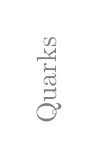
\begin{tikzpicture}
\node[rotate=90,opacity=0.5] at (-1,0.5) {Quarks};
\end{tikzpicture}
}
&
\begin{tikzpicture}
\node [mybox,anchor=west] (box) at (-1, 0) {};
\node[circle, inner sep=2pt, minimum size=0.3cm,draw=none,fill=blue!50] at (0.2, 0.1) { \Large{u} };
\node[anchor=west] at (-1,0.8) {\tiny{$2.4$ MeV/$c^2$}};
\node[anchor=west] at (-1,0) {\tiny{$2/3$}};
\node[anchor=west] at (-1,-0.5) {\tiny{$1/2$}};
\node at (0.4, -0.5) { up };
\end{tikzpicture}
&
\begin{tikzpicture}
\node [mybox,anchor=west] (box) at (-1, 0) {};
\node[circle, inner sep=2pt, minimum size=0.3cm,draw=none,fill=blue!50] at (0.2, 0.1) { \Large{c} };
\node[anchor=west] at (-1,0.8) {\tiny{$1.27$ GeV/$c^2$}};
\node[anchor=west] at (-1,0) {\tiny{$2/3$}};
\node[anchor=west] at (-1,-0.5) {\tiny{$1/2$}};
\node at (0.4, -0.5) { charm };
\end{tikzpicture}
&
\begin{tikzpicture}
\node [mybox,anchor=west] (box) at (-1, 0) {};
\node[circle, inner sep=2pt, minimum size=0.3cm,draw=none,fill=blue!50] at (0.2, 0.1) { \Large{t} };
\node[anchor=west] at (-1,0.8) {\tiny{$172.5$ GeV/$c^2$}};
\node[anchor=west] at (-1,0) {\tiny{$2/3$}};
\node[anchor=west] at (-1,-0.5) {\tiny{$1/2$}};
\node at (0.4, -0.5) { top };
\end{tikzpicture}
&
\begin{tikzpicture}
\node [mybox,anchor=west] (box) at (-1, 0) {};
\node[circle, inner sep=2pt, minimum size=0.3cm,draw=none,fill=blue!50] at (0.2, 0.1) { \Large{$\gamma$} };
\node[anchor=west] at (-1,0.8) {\tiny{$0$ MeV/$c^2$}};
\node[anchor=west] at (-1,0) {\tiny{$0$}};
\node[anchor=west] at (-1,-0.5) {\tiny{$1$}};
\node at (0.4, -0.5) { photon };
\end{tikzpicture}
&
\begin{tikzpicture}
\node [mybox,anchor=west] (box) at (-1, 0) {};
\node[circle, inner sep=2pt, minimum size=0.3cm,draw=none,fill=blue!50] at (0.2, 0.1) { \Large{H} };
\node[anchor=west] at (-1,0.8) {\tiny{$\sim 125$ GeV/$c^2$}};
\node[anchor=west] at (-1,0) {\tiny{$0$}};
\node[anchor=west] at (-1,-0.5) {\tiny{$0$}};
\node at (0.4, -0.5) { Higgs };
\end{tikzpicture}
\\
&
\begin{tikzpicture}
\node [mybox,anchor=west] (box) at (-1, 0) {};
\node[circle, inner sep=2pt, minimum size=0.3cm,draw=none,fill=blue!50] at (0.2, 0.1) { \Large{d} };
\node[anchor=west] at (-1,0.8) {\tiny{$4.8$ MeV/$c^2$}};
\node[anchor=west] at (-1,0) {\tiny{$-1/3$}};
\node[anchor=west] at (-1,-0.5) {\tiny{$1/2$}};
\node at (0.4, -0.5) { down };
\end{tikzpicture}
&
\begin{tikzpicture}
\node [mybox,anchor=west] (box) at (-1, 0) {};
\node[circle, inner sep=2pt, minimum size=0.3cm,draw=none,fill=blue!50] at (0.2, 0.1) { \Large{s} };
\node[anchor=west] at (-1,0.8) {\tiny{$104$ MeV/$c^2$}};
\node[anchor=west] at (-1,0) {\tiny{$-1/3$}};
\node[anchor=west] at (-1,-0.5) {\tiny{$1/2$}};
\node at (0.4, -0.5) { strange };
\end{tikzpicture}
&
\begin{tikzpicture}
\node [mybox,anchor=west] (box) at (-1, 0) {};
\node[circle, inner sep=2pt, minimum size=0.3cm,draw=none,fill=blue!50] at (0.2, 0.1) { \Large{b} };
\node[anchor=west] at (-1,0.8) {\tiny{$4.2$ GeV/$c^2$}};
\node[anchor=west] at (-1,0) {\tiny{$-1/3$}};
\node[anchor=west] at (-1,-0.5) {\tiny{$1/2$}};
\node at (0.4, -0.5) { bottom };
\end{tikzpicture}
&
\begin{tikzpicture}
\node [mybox,anchor=west] (box) at (-1, 0) {};
\node[circle, inner sep=2pt, minimum size=0.3cm,draw=none,fill=blue!50] at (0.2, 0.1) { \Large{g} };
\node[anchor=west] at (-1,0.8) {\tiny{$0$ MeV/$c^2$}};
\node[anchor=west] at (-1,0) {\tiny{$0$}};
\node[anchor=west] at (-1,-0.5) {\tiny{$1$}};
\node at (0.4, -0.5) { gluon };
\end{tikzpicture}
&
\multirow{3}{*}{
\hspace{-0.5cm}

\begin{tikzpicture}
\node[rotate=90,opacity=0.5] {Bosons};
\end{tikzpicture}
}
\\
&&&&&\\
\multirow{2}{*}{
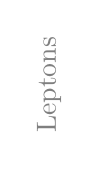
\begin{tikzpicture}
\node[rotate=90,opacity=0.5] at (-1,0.5) {Leptons};
\end{tikzpicture}
}&
\begin{tikzpicture}
\node [mybox,anchor=west] (box) at (-1, 0) {};
\node[circle, inner sep=2pt, minimum size=0.3cm,draw=none,fill=blue!50] at (0.2, 0.1) { \Large{e} };
\node[anchor=west] at (-1,0.8) {\tiny{$0.511$ MeV/$c^2$}};
\node[anchor=west] at (-1,0) {\tiny{$-1$}};
\node[anchor=west] at (-1,-0.5) {\tiny{$1/2$}};
\node at (0.4, -0.5) { electron };
\end{tikzpicture}
&
\begin{tikzpicture}
\node [mybox,anchor=west] (box) at (-1, 0) {};
\node[circle, inner sep=2pt, minimum size=0.3cm,draw=none,fill=blue!50] at (0.2, 0.1) { \Large{$\mu$} };
\node[anchor=west] at (-1,0.8) {\tiny{$105.7$ MeV/$c^2$}};
\node[anchor=west] at (-1,0) {\tiny{$-1$}};
\node[anchor=west] at (-1,-0.5) {\tiny{$1/2$}};
\node at (0.4, -0.5) { muon };
\end{tikzpicture}
&
\begin{tikzpicture}
\node [mybox,anchor=west] (box) at (-1, 0) {};
\node[circle, inner sep=2pt, minimum size=0.3cm,draw=none,fill=blue!50] at (0.2, 0.1) { \Large{$\tau$} };
\node[anchor=west] at (-1,0.8) {\tiny{$1.77$ GeV/$c^2$}};
\node[anchor=west] at (-1,0) {\tiny{$-1$}};
\node[anchor=west] at (-1,-0.5) {\tiny{$1/2$}};
\node at (0.4, -0.5) { tau };
\end{tikzpicture}
&
\begin{tikzpicture}
\node [mybox,anchor=west] (box) at (-1, 0) {};
\node[circle, inner sep=2pt, minimum size=0.3cm,draw=none,fill=blue!50] at (0.2, 0.1) { \Large{$Z$} };
\node[anchor=west] at (-1,0.8) {\tiny{$91.2$ GeV/$c^2$}};
\node[anchor=west] at (-1,0) {\tiny{$0$}};
\node[anchor=west] at (-1,-0.5) {\tiny{$1$}};
\node at (0.4, -0.5) { Z };
\end{tikzpicture}
&
\\
&
\begin{tikzpicture}
\node [mybox,anchor=west] (box) at (-1, 0) {};
\node[circle, inner sep=2pt, minimum size=0.3cm,draw=none,fill=blue!50] at (0.2, 0.1) { \Large{$\nu_e$} };
\node[anchor=west] at (-1,1.0) {\tiny{unknown}};
\node[anchor=west] at (-1,0.8) {\tiny{but $> 0$ eV/$c^2$}};
\node[anchor=west] at (-1,0) {\tiny{$0$}};
\node[anchor=west] at (-1,-0.5) {\tiny{$1/2$}};
\node at (0.4, -0.5) { electron };
\node at (0.2, -1) { neutrino };
\end{tikzpicture}
&
\begin{tikzpicture}
\node [mybox,anchor=west] (box) at (-1, 0) {};
\node[circle, inner sep=2pt, minimum size=0.3cm,draw=none,fill=blue!50] at (0.2, 0.1) { \Large{$\nu_\mu$} };
\node[anchor=west] at (-1,1.0) {\tiny{unknown}};
\node[anchor=west] at (-1,0.8) {\tiny{but $> 0$ eV/$c^2$}};
\node[anchor=west] at (-1,0) {\tiny{$0$}};
\node[anchor=west] at (-1,-0.5) {\tiny{$1/2$}};
\node at (0.4, -0.5) { muon };
\node at (0.2, -1) { neutrino };
\end{tikzpicture}
&
\begin{tikzpicture}
\node [mybox,anchor=west] (box) at (-1, 0) {};
\node[circle, inner sep=2pt, minimum size=0.3cm,draw=none,fill=blue!50] at (0.2, 0.1) { \Large{$\nu_\tau$} };
\node[anchor=west] at (-1,1.0) {\tiny{unknown}};
\node[anchor=west] at (-1,0.8) {\tiny{but $> 0$ eV/$c^2$}};
\node[anchor=west] at (-1,0) {\tiny{$0$}};
\node[anchor=west] at (-1,-0.5) {\tiny{$1/2$}};
\node at (0.4, -0.5) { tau };
\node at (0.2, -1) { neutrino };
\end{tikzpicture}
&
\begin{tikzpicture}
\node [mybox,anchor=west] (box) at (-1, 0) {};
\node[circle, inner sep=2pt, minimum size=0.3cm,draw=none,fill=blue!50] at (0.2, 0.1) { \Large{$W$} };
\node[anchor=west] at (-1,0.8) {\tiny{$80.4$ GeV/$c^2$}};
\node[anchor=west] at (-1,0) {\tiny{$\pm 1$}};
\node[anchor=west] at (-1,-0.5) {\tiny{$1$}};
\node at (0.2, -0.5) { $W$ };
\end{tikzpicture}
&
\begin{tikzpicture}
\node [mybox,anchor=west] (box) at (-1, 0) {};
\node[circle, inner sep=0pt, minimum size=0.3cm,draw=none,fill=blue!50] at (0.4, 0.1) { \tiny{symbol} };
\node[anchor=west] at (-1,0.8) {\tiny{mass}};
\node[anchor=west] at (-1,0) {\tiny{charge}};
\node[anchor=west] at (-1,-0.5) {\tiny{spin}};
\node at (0.4, -0.5) { name };
\end{tikzpicture}
\begin{tikzpicture}[remember picture, overlay]
\node[opacity=0.6] at (-0.8,2cm) {Legend};
\end{tikzpicture}
\\
\end{tabular}
\begin{tikzpicture}[remember picture,overlay]
\draw[green,fill=none,thick, rounded corners] (-6.8cm,5.6cm)  rectangle (2cm,0);
\draw[green,fill=none,thick, rounded corners] (-6.8cm,11.3cm)  rectangle (2cm,5.8cm);
\coordinate (A1) at (2.1cm,11.3cm);
\coordinate (A2) at (2.1cm,0cm);
\coordinate (A3) at (4.5cm,0cm);
\coordinate (A4) at (4.5cm,2.9cm);
\coordinate (A5) at (7.0cm,2.9cm);
\coordinate (A6) at (7.0cm,11.3cm);
\draw[green,fill=none,thick, rounded corners] (A1) -- (A2) -- (A3) -- (A4) -- (A5) -- (A6) -- (A1);
\draw[red!50!black,fill=none,very thick, rounded corners] (-6.9cm,11.5cm)  rectangle (7.1cm,-0.1cm);
\end{tikzpicture}
\label{tab:smpart}
\end{table}

The electroweak interactions couple differently to right-handed and left-handed fields, which are grouped differently in $SU(2)$ singlets and doublets
representations~\cite{qft}, as follows:

\begin{table}[H]
\centering
\begin{tabular}{ >{\centering\arraybackslash}m{2cm} >{\centering\arraybackslash}m{2cm} >{\centering\arraybackslash}m{2cm} >{\centering\arraybackslash}m{2cm} >{\centering\arraybackslash}m{2cm} >{\centering\arraybackslash}m{2cm}}
$\begin{pmatrix}  u \\ d \end{pmatrix}_L$ & $\begin{pmatrix} c \\ s \end{pmatrix}_L$ & $\begin{pmatrix} t \\ b \end{pmatrix}_L$ & $\begin{pmatrix} \nu_e \\ e \end{pmatrix}_L$ & $\begin{pmatrix} \nu_\mu \\ \mu \end{pmatrix}_L$ & $\begin{pmatrix} \nu_\tau \\ \tau \end{pmatrix}_L$ \\
&&&&&\\
$u_R$ & $c_R$ & $t_R$ & & &  \\
&&&&&\\
$d_R$ & $s_R$ & $b_R$ & $e_R$ & $\mu_R$ & $\tau_R$ \\
\end{tabular}
\label{eq:field_rep}
\end{table}
in which the left-handed fields have the $L$ subscript and they are arranged in the doublet representation of the $SU(2)$ group, while the right-handed
particles are arranged in the singlet representation with the $R$ subscript. The fields have quantum numbers associated to their interaction in the SM, which will
be detailed in the next subsection. For completeness, the fields' quantum numbers for their electroweak interactions is described here.
The fields arranged in $SU(2)$ doublets have their third component of the isospin $I_3 = \pm \frac{1}{2}$, with the positive value associated with the up-type quarks and
neutrinos and the negative value, to down-type quarks, electron, muon and tauon. The right-handed fields have $I_3 = 0$. The up-type quarks have an electric
charge $Q = + \frac{2}{3}$ and the down-type quarks have $Q = - \frac{1}{3}$. Neutrinos have neutral electric charge and electron, muons and tau have charge $Q = -1$.
A third quantum number relates to the weak hypercharge $Y$ and it is associated such that the relation $Q = I_3 + Y$ is respected~\footnote{Some authors use the $Q = I_3 + Y/2$
convention instead. This document follows the convention in~\cite{qft}.}.

Note that there is no mention of the right-handed neutrinos in this discussion, which is
how the Standard Model was initially presented, since the neutrinos were assumed to be massless. Experimental evidence suggests that neutrinos are not massless, though,
and the theory should be changed in that respect~\cite{neutrino1,neutrino2,neutrino3}. This is not a central point in the analyses that follow, so it will not be
further discussed in this document.

The SM is described by a Lagrangian density that can be separated into a gauge term, a matter term, a Yukawa term and a Higgs term~\cite{Incandela:2009pf}:

\begin{equation*}
\displaystyle
\mathcal{L}_{\textrm{SM}} = \mathcal{L}_{\textrm{Matter}} + \mathcal{L}_{\textrm{Gauge}} + \mathcal{L}_{\textrm{Yukawa}} + \mathcal{L}_{\textrm{Higgs}}.
\end{equation*}
The matter Lagrangian contains the kinetic energy of the quarks and leptons and their interactions, which is given by their coupling to the gauge fields.
The gauge term of the Lagrangian includes the kinetic energy of gauge fields for strong and electroweak
interactions, leading to the description of their propagation mechanism.
The interaction of the Higgs field with the quarks and leptons is done by the
Yukawa interaction terms of the Lagrangian, which provides a dynamical mechanism by which the
particles acquire mass.
Finally, the Higgs field sector contains the Higgs kinetic energy and the
Higgs potential, which causes a non-zero vacuum expectation value for the Higgs field.

\subsection{Matter fields and electroweak interactions}

The matter fields are generically represented as spinors $\mathbf{\Psi}$, which could be incorporated as a free field
with a single kinetic term~\cite{topreview_wagner,qft}:

\begin{equation}
\displaystyle
\mathcal{L}_0 = i \bar{\mathbf{\Psi}} \gamma^{\mu} \partial_\mu \mathbf{\Psi},
\label{eq:free_lagrangian}
\end{equation}
in which $\gamma^\mu$ is defined as a set of four matrices that satisfy $\{\gamma^\mu,\gamma^\nu\} \equiv \gamma^\mu \gamma^\nu + \gamma^\nu \gamma^\mu = 2 g^{\mu \nu} I_4$,
where $g^{\mu \nu}$ is the Minkowski metric~\cite{qft} and $I_4$ is the $4 \times 4$ identity matrix. The Dirac adjoint is defined as
$\bar{\mathbf{\Psi}} \equiv \mathbf{\Psi}^\dagger \gamma^0$, where $\mathbf{\Psi}^\dagger$ represents the Hermitian adjoint of $\mathbf{\Psi}$.

This results in a field that satisfies the Dirac equation~\cite{qft}, but does not include the interactions in the theory.
As was mentioned previously, the Standard Model demands gauge invariance over a set of Lie groups, particularly over
$SU(2)_L \times U(1)_Y$ for the electroweak force. This gauge invariance is implemented by demanding the invariance of the Lagrangian 
%(or, more generally, the action)
on the transformation:

%\begin{eqnarray}
%\displaystyle
%\mathbf{\Psi}_L & \rightarrow & e^{i g \mathbf{\alpha}(x) \mathbf{T} + i g^{\prime} \beta(x) Y(\mathbf{\Psi}_L)} \mathbf{\Psi}_L , \nonumber\\
%\mathbf{\Psi}_R & \rightarrow & e^{i g^{\prime} \beta(x) Y(\mathbf{\Psi_R})} \mathbf{\Psi}_R ,
%\label{eq:gauge_electroweak}
%\end{eqnarray}

\begin{eqnarray}
\displaystyle
\mathbf{\Psi}_L & \rightarrow & e^{i \mathbf{\alpha}(x) \cdot \mathbf{T}} \mathbf{\Psi}_L , \nonumber\\
\mathbf{\Psi}_R & \rightarrow & \mathbf{\Psi}_R ,
\label{eq:gauge_su2}
\end{eqnarray}
for the $SU(2)_L$ symmetry and:

\begin{eqnarray}
\displaystyle
\mathbf{\Psi}_L & \rightarrow & e^{i \beta(x) Y(\mathbf{\Psi_L}) } \mathbf{\Psi}_L , \nonumber\\
\mathbf{\Psi}_R & \rightarrow & e^{i \beta(x) Y(\mathbf{\Psi_R}) } \mathbf{\Psi}_R ,
\label{eq:gauge_su1}
\end{eqnarray}
for the $U(1)_Y$ symmetry.
In these equations, $\mathbf{\Psi}_R$ and $\mathbf{\Psi}_L$ represent the right-handed and left-handed fields respectively;
$Y(\mathbf{\Psi})$ is the weak hypercharge of the field $\mathbf{\Psi}$;
$\mathbf{T} = \begin{pmatrix} T^1 & T^2 & T^3 \end{pmatrix}^{T}$ is the weak isospin operator~\footnote{The symbol $T$ in the superscript indicates that the transverse of the matrix is to be taken.}, whose components are the generators of the $SU(2)_L$ transformation and can be
written as $T^a = \frac{1}{2} \sigma^a$ (where $\sigma^a$ are the Pauli matrices);
$\mathbf{\alpha}(x)$
is an arbitrary three-component vector of functions of the space-time; $\beta(x)$ is an arbitrary function
of the space-time. The Lagrangian can be made invariant over these transformations, by substituting the $\partial_\mu$ in $\mathcal{L}_0$ by the covariant derivative
$D_\mu$:

\begin{equation}
\displaystyle
D_{\mu} \mathbf{\Psi} = (\partial_\mu - i g \mathbf{W}_\mu \cdot \mathbf{T} - i g^{\prime} Y(\mathbf{\Psi}) B_\mu ) \mathbf{\Psi} ,
\label{eq:dcov}
\end{equation}
in which $g$ and $g^{\prime}$ are coupling constants and
gauge fields~\footnote{In this document, the term ``gauge fields''
is used to refer to these objects. In some (mostly mathematical texts),
these objects are called ``connections''.}
$\mathbf{W} = \begin{pmatrix} W^1 & W^2 & W^3 \end{pmatrix}$ and $B$ are incorporated~\footnote{Note that in $\mathbf{W}_\mu \cdot \mathbf{T}$,
the $\mathbf{A} \cdot \mathbf{B}$ operation is defined as $\mathbf{A} \cdot \mathbf{B} \equiv A^a B^a \equiv \sum_a A^a B^a$.}.
%$I_3(\mathbf{\Psi})$ is the third component of the weak isospin of the
%field $\mathbf{\Psi}$ (note that the $|2 I_3(\mathbf{\Psi})|$ is zero for the right-handed fields and one for the left-handed fields).
It is implicit
that only the left-handed fields couple to the $SU(2)_L$ generators term.
%Furthermore, to guarantee gauge invariance, the gauge fields
%transform according to:
%
%\begin{eqnarray}
%\displaystyle
%W^a_\mu \rightarrow W^a_\mu T^a + \frac{1}{g}(\partial_\mu \alpha^a(x)) + i \epsilon^{abc} W^b_\mu \alpha^c(x) \nonumber \\
%B_\mu \rightarrow B_\mu + \frac{1}{g^\prime}\partial_\mu \beta(x) .
%\label{eq:wbgauge}
%\end{eqnarray}

The usage of the covariant derivative $D_{\mu}$ includes
the coupling of the matter fields with the $\mathbf{W}$ and $B$ fields in the kinetic term of the Lagrangian.
The gauge fields have their kinetic terms added in the gauge part of the Lagrangian as $- \frac{1}{4} W_{\mu \nu}^a W^{\mu \nu,a} - \frac{1}{4} B_{\mu \nu} B^{\mu \nu}$, with:

\begin{eqnarray}
\displaystyle
W^i_{\mu \nu}&=&\partial_\mu W^i_\nu -  \partial_\nu W^i_\mu + g \epsilon^{ijk} W^{j}_\mu W^{k}_\nu , \nonumber \\
B_{\mu \nu}&=& \partial_\mu B_\mu - \partial_\nu B_\mu.
\label{eq:WBfields}
\end{eqnarray}
The mass eigenstates of the electroweak fields are not $W^1$, $W^2$, $W^3$ and $B$,
but a linear transformation of them, represented as $W^+$, $W^-$, $Z$ and the photon field $A$. The electroweak fields acquire mass through the mechanism mentioned
in Section~\ref{subsec:higgs}. It is convenient to treat the electroweak fields in their mass eigenstates, given by:
\begin{eqnarray}
\displaystyle
W^+_\mu & = & \frac{W^1_\mu - iW^2_\mu}{\sqrt{2}}, \\
W^-_\mu & = & \frac{W^1_\mu + iW^2_\mu}{\sqrt{2}}, \\
\begin{pmatrix} Z_\mu \\ A_\mu \end{pmatrix} & = & \begin{pmatrix} \cos \theta_W & -\sin \theta_W \\ \sin \theta_W & \cos \theta_W \end{pmatrix} \begin{pmatrix} W^3_\mu \\ B_\mu \end{pmatrix},
\label{eq:electroweak_transf}
\end{eqnarray}
where the weak mixing angle $\theta_W$ is defined such that $g \sin \theta_W = g^{\prime} \cos \theta_W = e$, where $e$ is the charge of the electron.

\subsection{Quantum Chromodynamics}

Another force included in the Standard Model is the strong interaction, which is in the domain of Quantum Chromodynamics (QCD).
The strong interaction is incorporated by demanding invariance of the Lagrangian due to a $SU(3)_C$ local gauge transformation:

\begin{equation}
\displaystyle
\mathbf{\Psi} \rightarrow e^{i \mathbf{\kappa}(x) \cdot \mathbf{t}} \mathbf{\Psi},
\label{eq:gauge_qcd}
\end{equation}
in which $\mathbf{t} = \begin{pmatrix} t^1 & t^2 & t^3 & t^4 & t^5 & t^6 & t^7 & t^8 \end{pmatrix}^T$ are the $SU(3)$ generators
and
$\mathbf{\kappa}(x)$ is an arbitrary eight-component vector of functions of the space-time.
The gauge invariance requirement is incorporated in the
Standard Model, by including the gluon field in the covariant derivative described previously (Equation~\ref{eq:dcov}):

\begin{eqnarray}
\displaystyle
D_{\mu} \mathbf{\Psi}&=&(\partial_\mu - i g \mathbf{W}_\mu \cdot \mathbf{T} - i g^{\prime} Y(\mathbf{\Psi}) B_\mu ) \mathbf{\Psi} \nonumber \\
&& - (i g_S \mathbf{G}_\mu \cdot \mathbf{t}) \mathbf{\Psi},
\label{eq:dcov_qcd}
\end{eqnarray}
in which the $\mathbf{G}$ is an eight-component vector that represents the gluon fields
%(which transform similarly to the $\mathbf{W}$ and $B$ fields mentioned
%in the previous section, under the gauge transformation of
%the matter fields)
and $g_S$ is the strong force coupling constant.
It is also common to write the strong coupling constant
as a function of $\alpha_S = g_S^2/4\pi$.
This addition to the covariant derivative (for quarks) allows the quark fields to emit and absorb gluons, through the $i \bar{\mathbf{\Psi}} \gamma^\mu D_\mu \mathbf{\Psi}$ term
of the Lagrangian.
The dynamics of the new gluon fields can be included by an extra kinetic term $- \frac{1}{4} F_{\mu\nu}^a F^{\mu\nu,a}$, where:
\begin{eqnarray}
\displaystyle
F_{\mu\nu}^a = \partial_\mu G^a_\nu - \partial_\nu G^a_\mu + g_S f^{abc} G^b_\mu G^c_\nu.
\label{eq:gluon_gauge}
\end{eqnarray}

Calculations in a Quantum Field Theory can be done by ignoring the interaction terms for the fields at first, and including them at a later stage as a perturbation
to the free field solutions, taking only the first terms in the expansion~\cite{qft}. When calculating the terms of the perturbative expansion in both QCD and the electroweak
theory, there are ultraviolet~\cite{qft} divergencies~\footnote{We use the jargon ``ultraviolet divergencies'' here to refer to divergencies caused by high energies
and ``infrared divergencies'' to refer to divergencies caused by low energies.}, which lead to a non-physical prediction for some observables.
In ``renormalisable'' theories~\cite{qft},
such as QCD and the electroweak theory, these divergencies happen only in a countable number of interaction diagrams and they can be removed from the physical
observables by redefining the Lagrangian so that a new set of parameters have these divergencies ``subtracted''. The process of redefining the model in such a way
that these divergencies are removed from physical observables is called ``renormalisation''~\cite{qft}. It can be done in multiple ways, leading
to different ``renormalisation schemes''~\cite{qft}. The renormalised parameters of the theory depend on a ``renormalisation scale'' $\mu_R$, although the physical
observables do not depend on this scale.

A consequence of this procedure in QCD is that the
renormalised coupling constant $\alpha_S$ depends on the scale $\mu_R$ and on the (squared) momentum transfer
in a QCD interaction $- Q^2$. For low energies, QCD has a non-perturbative behaviour
and the perturbative expansion cannot be made. In such situations, other tools exist to study the QCD theory, such as Lattice QCD~\cite{latticeqcd}.
For higher energies though, the renormalised QCD coupling constant $\alpha_S(\mu_R)$ is such that the perturbative expansion is valid, as it can be
seen in its leading-order approximation:

\begin{equation}
\alpha_S(Q^2) = \frac{\alpha_S(\mu_R^2)}{1 + (b_0 \alpha_S(\mu_R^2)/2\pi) \ln(Q^2/\mu_R^2)},
\label{eq:alphas}
\end{equation}
where $b_0$ is a positive coeficient~\cite{qft} (assuming the approximation of massless quarks) and, therefore, for high enough values of $Q^2$ QCD can be
analysed using perturbation theory, in what is often called ``pQCD'' (for ``perturbative QCD''). pQCD can be used for interactions involving momentum transfers well
above the $\Lambda_{\textrm{QCD}} \sim 200\mev$ experimental threshold, for example, above $Q = 1\gev$, where $\alpha_S(Q^2) \sim 0.4$~\cite{qft}.

% MENTION: pQCD can be studied in high energy experiments
With this behaviour (often called ``asymptotic freedom''), the high energy environment is an ideal scenario to study QCD, since perturbation theory
provides an excellent tool to study its interactions. One of the key topics of this thesis is to
measure the effect of QCD radiation at high energies, produced in association with
the top quark.

For smaller $Q^2$ though, the coupling constant increases and QCD grows even stronger. In this scenario, the strong force also becomes stronger as the distance between the
particles increase. At sufficiently large distances, the potential energy between the quarks, produced by QCD, is strong enough to produce new quark pairs. This effect, called
``confinement'' does not allow one to measure a free quark: they are always in colourless bound states. What can be measured in the detector, therefore, is never a quark itself,
but its byproducts. For this reason, the QCD radiation measured in this document is detected as a set of particles in a region of the experiment, and not as bare quarks
or gluons.

\subsection{Electroweak symmetry breaking mechanism}
\label{subsec:higgs}

%MENTION: HIGGS, yukawa coupling
The sectors of the Standard Model discussed previously include fields for the matter particles and the gauge boson fields $W^{\pm}$, $Z$, the photon and the gluons.
While the photon and the gluons are massless, the electron, muon, tauon, the six quarks, the $W^{\pm}$ and $Z$ are not~\footnote{As it was already
mentioned, there is evidence that supports that neutrinos
are not massless, although their mass is much smaller than any other particle in the Standard Model. They are assumed massless here though, since their mass is much smaller
than what can be experimentally verified in the ATLAS detector (Chapter~\ref{chp:atlas}) and their non-zero mass does not affect the process of the measurement and searches
shown in this document.}. Including mass terms in the Lagrangian which resemble $m\bar{\mathbf{\Psi}}\mathbf{\Psi}$ or $m V_\mu V^\mu$ can be
shown to violate the gauge invariance of the
SM~\cite{qft}.

A mechanism has been devised, called the ``Englert –- Brout -– Higgs -– Guralnik -– Hagen -– Kibble mechanism''~\footnote{Other
names are also used for it, including the ``Higgs mechanism'',
the ``Brout -- Englert -- Higgs mechanism'' and the ``ABEGHHK'tH mechanism'' (for Anderson, Brout, Englert, Guralnik, Hagen, Higgs, Kibble and 't Hooft).}, which introduces
a scalar field~\cite{qft} $\mathbf{\phi} = \frac{1}{\sqrt{2}} \begin{pmatrix} \phi^+ \\ \phi^0 \end{pmatrix}$, which is an $SU(2)$ doublet. This field couples to the gauge bosons described
previously due to its kinetic term and it couples to itself through the potential $V(\mathbf{\phi})$:

\begin{eqnarray}
\mathcal{L}_\textrm{Higgs}&=&D_\mu\mathbf{\phi}^\dagger D^\mu\mathbf{\phi} - V(\mathbf{\phi}) \textrm{ , where: } \\
V(\mathbf{\phi})&=&-\mu^2\mathbf{\phi}^\dagger \mathbf{\phi} + \frac{\lambda}{2} (\mathbf{\phi}^\dagger \mathbf{\phi})^2,
\label{eq:higgs}
\end{eqnarray}
in which $\mu^2$ and $\lambda$ are parameters of the model. For $\mu^2 > 0$, the potential has a maximum at the origin
and minima at $<\phi>_0 = v = \Big(\frac{\mu^2}{\lambda}\Big)^{1/2}$.
While the point at zero is unstable, the minima are stable and sets the vacuum expectation
value for the field.

Gauge invariance is preserved in the Lagrangian, through this mechanism, and
the coupling of this field to the fermion and gauge boson fields dynamically generates their mass.
The interaction terms between the Higgs boson and the matter fields are added in the Yukawa sector of the Lagrangian.
Note as well that the gauge bosons have their masses included by the $|D^\mu\mathbf{\phi}|^2$ term of the Lagrangian.

A further effect of this spontaneous symmetry breaking of the Lagrangian is the existence of a Higgs boson particle with mass $\sqrt{2} \mu$.
A Higgs boson has recently been verified experimentally at the LHC~\cite{higgs_atlas,higgs_cms} and it is still under study.
Note that the masses associated to the matter fields are related to their coupling to the Higgs field, therefore, the most massive particle
in the Standard Model, the top quark, would be strongly connected to the Higgs boson.

\section{The Standard Model and the top quark}

The top quark, discovered in 1995 at Fermilab, has a few interesting properties which are going to be explored in this document. To discuss the top quark, a few
remarks will be made first on a few elements of the Standard Model interactions.

The electroweak interaction can be expressed in terms of the $W^{\pm}$, $Z$ and photon fields, but only the $W^{\pm}$ currents change fermions'
flavours at tree level, while the neutral bosons do not change the fermion flavour. Decays of particles which change flavour
and include neutral currents are allowed in the SM in diagrams with loops, but these are highly suppressed~\cite{gim}.
One important characteristic of the SM is that the $W^{\pm}$ bosons do not act on the quark fields described previously, but on
a linear combination of quark fields, with weights given by the CKM matrix~\cite{cabbibo,kobayashi,smsummary}.
It is instructive to verify how the charged currents $J^{\mu}_W$ (and its adjoint $J^{\mu \dagger}_W$) and the neutral currents $J^\mu_Z$ and $J^\mu_{\textrm{EM}}$
show the interaction between the fermions and the $W^{\pm}$-bosons
after the electroweak symmetry breaking~\cite{qft,smsummary}:

\begin{equation}
\displaystyle
\mathcal{L}_{\textrm{SM}} \supset g \Big( W_\mu^- J^{\mu}_W + W_\mu^+ J^{\mu \dagger}_W + Z_\mu J_Z^\mu \Big) + e A_\mu J^\mu_{\textrm{EM}},
\label{eq:w_int}
\end{equation}
where the symbol $\supset$ indicates that the Lagrangian can be rewritten so that this is one of its terms~\cite{qft}.
The currents can be defined as follows~\cite{qft}:

\begin{eqnarray}
\displaystyle
J^{\mu \dagger}_W&=&\frac{1}{\sqrt{2}} ( \bar{\nu}_L \gamma^{\mu} \ell_L + \bar{U}_L \gamma^{\mu} V_{CKM} D_L ), \\
J^{\mu}_Z&=&\frac{1}{\cos \theta_W} \Big[ \bar{\nu}_L \gamma^\mu (\frac{1}{2}) \nu_L + \bar{\ell}_L \gamma^\mu (-\frac{1}{2} + \sin^2\theta_W)\ell_L + \bar{\ell}_R \gamma^\mu (\sin^2 \theta_W)\ell_R + \nonumber \\
 && + \bar{U}_L \gamma^\mu (\frac{1}{2} - \frac{2}{3} \sin^2 \theta_W) U_L + \bar{U}_R \gamma^\mu (-\frac{2}{3} \sin^2 \theta_W) U_R + \nonumber \\
&& + \bar{D}_L \gamma^\mu (-\frac{1}{2} + \frac{1}{3} \sin^2 \theta_W) D_L + \bar{D}_R \gamma^\mu (\frac{1}{3} \sin^2 \theta_W) D_R \Big] , \\
J^{\mu}_{\textrm{EM}}&=&\bar{\ell} \gamma^\mu (-1) \ell + \bar{U} \gamma^\mu (+\frac{2}{3}) U + \bar{D} \gamma^\mu (-\frac{1}{3}) D \\
\label{eq:w_current}
\end{eqnarray}
in which the matter fields are arranged for convenience such that (the same symbols are used to identify the particles as in Table~\ref{tab:smpart})~\footnote{The symbol T in the superscript represents
the transpose of the matrices.}:

\begin{eqnarray}
\displaystyle
\nu_L &= &\begin{pmatrix} \nu_e & \nu_\mu & \nu_\tau\end{pmatrix}^T_L , \\
\ell_L &= & \begin{pmatrix} e & \mu & \tau \end{pmatrix}^T_L ,\\
\ell_R &= & \begin{pmatrix} e & \mu & \tau \end{pmatrix}^T_R ,\\
U_L&=&\begin{pmatrix} u & c & t\end{pmatrix}^T_L ,\\
D_L&=&\begin{pmatrix} d & s & b\end{pmatrix}^T_L ,\\
U_R&=&\begin{pmatrix} u & c & t\end{pmatrix}^T_R ,\\
D_R&=&\begin{pmatrix} d & s & b\end{pmatrix}^T_R ,\\
\ell &=& \ell_L + \ell_R , \\
U&=&U_L+U_R , \\
D&=&D_L+D_R ,
\label{eq:fields}
\end{eqnarray}
and the
$V_{CKM}$ matrix is the CKM~\cite{cabbibo,kobayashi} matrix given by:

\begin{equation}
\displaystyle
V_{CKM} = \begin{pmatrix} V_{ud} & V_{us} & V_{ub} \\ V_{cd} & V_{cs} & V_{cb} \\ V_{td} & V_{ts} & V_{tb} \end{pmatrix}.
\label{eq:ckm}
\end{equation}

An important side effect of this structure for the Lagrangian density is that the coupling of the charged currents to the quarks includes elements of the $V_{CKM}$ matrix,
which have been experimentally measured~\cite{pdg2012}.
A key characteristic of the CKM matrix~\cite{pdg2012} is that it has a $|V_{tb}|$ element very close to one, while
the elements $|V_{td}|$ and $|V_{ts}|$ are very close to zero.
The Feynman diagram vertex for the interaction between
the top quark and the $W$-boson involves a $|V_{tb}|$ contribution which enhances the decay of the top quark into a $W$-boson and a $b$-quark, while the small
values of the other elements in the same row suppress the decay of the top quark into the other flavours. In fact, the branching ratio of top
decays into a $W$-boson and a $b$-quark
has been measured to be $0.99 ^{+0.09}_{-0.08}$ (see~\cite{pdg2012}).

Furthermore, the neutral currents that describe the interaction of the $Z$-boson and the photon field with the quarks do not change the flavour
of the fermions~\cite{gim}, so that at tree-level, the top quark cannot decay into another quark interacting through a $Z$-boson or a photon. It can decay using neutral currents
through diagrams including loops, but these are highly suppressed, compared to the charged current tree-level diagram.
There are analyses that search for higher rates for a single-top production through Flavour Changing Neutral Currents (FCNC) and the current limits are given by the
ATLAS search~\cite{fcnc_atlas}, which has shown good agreement between data and the SM. The current cross section limit on the FCNC single top production is
$\sigma_{qg \rightarrow t} \times \textrm{Br}(t \rightarrow Wb) < 3.9 \pb$.

Also, the top quark has a lifetime of $\sim 5 \times 10^{-25}$ s~\cite{topcollider,Incandela:2009pf}, which is smaller than the characteristic formation time
of hadrons $\tau_{\textrm{form}} \sim 1/\Lambda_{QCD} \sim 3 \times 10^{-24}$ s~\cite{Incandela:2009pf}, where $\Lambda_{QCD}$ is the scale at which QCD becomes non-pertubative. This means that the top quark does not hadronise and that its decay happens almost
exclusively through the $t \rightarrow W b$ channel at tree-level, with other contributions being suppressed.

A study of the top quark radiation allows for a deeper
understanding of the Standard Model, particularly the QCD interaction. It also helps understanding and verifying the Standard Model description of this
quark.
More information can be found in a review of the Standard Model with a focus in the top quark and its discovery, in~\cite{Incandela:2009pf}.

\section{Top-antitop pair generation at the LHC}

The top quark is produced predominantly in the LHC proton-proton collisions through
strong interactions, paired with its anti-quark, as it is shown in Figure~\ref{fig:ttbar}.
The top pair production in the Tevatron experiments~\cite{top_tevatron,PhysRevLett.74.2626,PhysRevLett.74.2632}, which
collide protons and antiprotons, is dominated ($\sim 85\%$ of the cases) by
the quark-antiquark diagram (c) in Figure~\ref{fig:ttbar}, while in the LHC, the gluon-gluon diagrams (a), (b) and (d) have the dominant
contributions ($\sim 90\%$ of the cases).
The result of a full calculation of the top pair production cross
section can be seen in the review in~\cite{topreview_wagner}.

\begin{figure}[ht]
\centering
\subfloat[a]{
\begin{fmffile}{gggtt1}
  \begin{fmfgraph*}(40,25)
    % Note that the size is given in normal parentheses % instead of curly brackets.
    % Define external vertices from bottom to top
    \fmfleft{i1,i2}
    \fmfright{o1,o2}

    \fmflabel{$g$}{i1}
    \fmflabel{$g$}{i2}
    \fmflabel{$\bar{t}$}{o1}
    \fmflabel{$t$}{o2}

    \fmf{curly}{i1,v1,i2}
    \fmf{fermion}{o1,v2,o2}
    \fmf{curly,label=$g$}{v1,v2}

  \end{fmfgraph*}
\end{fmffile}
}
\subfloat[b]{
\begin{fmffile}{gggtt2}
  \begin{fmfgraph*}(40,25)
    % Note that the size is given in normal parentheses % instead of curly brackets.
    % Define external vertices from bottom to top
    \fmftop{i1,o1}
    \fmfbottom{i2,o2}

    \fmflabel{$g$}{i1}
    \fmflabel{$g$}{i2}
    \fmflabel{$t$}{o1}
    \fmflabel{$\bar{t}$}{o2}

    \fmf{curly}{i1,v1}
    \fmf{fermion}{v1,o1}
    \fmf{curly}{i2,v2}
    \fmf{fermion}{o2,v2}
    \fmf{fermion}{v2,v1}

    \fmffixedy{0}{o1,v1}
    \fmffixedy{0}{o2,v2}

  \end{fmfgraph*}
\end{fmffile}
}
\subfloat[c]{
\begin{fmffile}{gggtt3}
  \begin{fmfgraph*}(40,25)
    % Note that the size is given in normal parentheses % instead of curly brackets.
    % Define external vertices from bottom to top
    \fmfleft{i1,i2}
    \fmfright{o1,o2}

    \fmflabel{$q$}{i1}
    \fmflabel{$\bar{q}$}{i2}
    \fmflabel{$\bar{t}$}{o1}
    \fmflabel{$t$}{o2}

    \fmf{fermion}{i1,v1,i2}
    \fmf{fermion}{o1,v2,o2}
    \fmf{curly,label=$g$}{v1,v2}

  \end{fmfgraph*}
\end{fmffile}
}
\vspace*{1.0cm}
\subfloat[d]{
\begin{fmffile}{gggtt4}
  \begin{fmfgraph*}(40,25)
    % Note that the size is given in normal parentheses % instead of curly brackets.
    % Define external vertices from bottom to top
    \fmfleft{i1,i2}
    \fmfright{o2,o1}

    \fmflabel{$g$}{i1}
    \fmflabel{$g$}{i2}
    \fmflabel{$\bar{t}$}{o2}
    \fmflabel{$t$}{o1}

    \fmf{curly}{i1,v1}
    \fmf{fermion}{v1g,o1}
    \fmf{plain}{v1,v1g}
    \fmf{curly}{i2,v2}
    \fmf{fermion}{o2,v2g}
    \fmf{plain}{v2,v2g}
    \fmf{fermion}{v2,v1}

    \fmffixedy{0}{o1,v2}
    \fmffixedy{0}{o2,v1}

  \end{fmfgraph*}
\end{fmffile}
}
\vspace*{0.5cm}
\caption{Top-antitop main production diagrams at the LHC, at tree-level.}
\label{fig:ttbar}
\end{figure}


As mentioned previously, due to the large value of the $|V_{tb}|$ matrix element, each
top quark decays almost exclusively to $t \rightarrow W b$.
The $W$ boson may then decay leptonically, into a lepton and a neutrino,
or hadronically, into quarks, producing jets in the detector.
This is shown, schematically, in Figure~\ref{fig:topdecay}.

\begin{figure}[ht]
\centering
\begin{fmffile}{topdecay}
  \begin{fmfgraph*}(60,30)
    % Note that the size is given in normal parentheses % instead of curly brackets.
    % Define external vertices from bottom to top
    \fmfleft{it}
    \fmfright{ob,o2,o1}

    \fmflabel{$t$}{it}
    \fmflabel{$l$,$q^{\prime}$}{o2}
    \fmflabel{$\bar{\nu}$,$\bar{q}$}{o1}
    \fmflabel{$b$}{ob}

    \fmf{fermion}{it,v1,ob}
    \fmf{photon,label=$W$}{v1,v2}
    \fmf{fermion}{o1,v2,o2}

  \end{fmfgraph*}
\end{fmffile}
\vspace*{0.5cm}
\caption{Top quark decays}
\label{fig:topdecay}
\end{figure}

These decays create three different channels of study of the $t\bar{t}$ system:

\begin{itemize}
  \item $t\bar{t} \rightarrow \ell \ell \nu \nu b b$: the dilepton channel, which assumes that both $W$ bosons decay to leptons and neutrinos;
  \item $t\bar{t} \rightarrow \ell \nu b b j j$: the single lepton channel, which assumes that one $W$ boson decays to lepton and a neutrino,
        while the other one decays hadronically;
  \item $t\bar{t} \rightarrow b b j j j j$: the all-hadronic channel, which assumes that both $W$ bosons decay hadronically.
\end{itemize}
This thesis concentrates on the single lepton (or ``semileptonic'') channel.

The top quark may also be produced separately from an antitop, by the production diagrams
shown in Figure~\ref{fig:singletop}. These productions have lower
cross sections than the $t\bar{t}$ system production in the LHC. Note that all diagrams require a $W$ boson interaction, that is,
the electroweak interaction must be present, while top pairs are produced through the strong interactions.

\begin{figure}[ht]
\centering
\begin{fmffile}{stop1}
  \begin{fmfgraph*}(50,30)
    % Note that the size is given in normal parentheses % instead of curly brackets.
    % Define external vertices from bottom to top
    \fmftop{iq,oq}
    \fmfbottom{ig,ob}
    \fmfright{ot}

    \fmflabel{$g$}{ig}
    \fmflabel{$q$}{iq}
    \fmflabel{$\bar{b}$}{ob}
    \fmflabel{$t$}{ot}
    \fmflabel{$q\prime$}{oq}

    \fmf{fermion}{iq,vvq,oq}
    \fmf{photon,label=$W$}{vvb2,vvq}
    \fmf{fermion}{ob,vvb}
    \fmf{fermion}{vvb,vvb2}
    \fmf{fermion}{vvb2,ot}
    \fmf{curly}{ig,vvb}

  \end{fmfgraph*}
\end{fmffile} \hspace*{1cm}
\begin{fmffile}{stop2}
  \begin{fmfgraph*}(50,25)
    % Note that the size is given in normal parentheses % instead of curly brackets.
    % Define external vertices from bottom to top
    \fmftop{iq,oq}
    \fmfbottom{ib,ot}

    \fmflabel{$q$}{iq}
    \fmflabel{$q\prime$}{oq}
    \fmflabel{$b$}{ib}
    \fmflabel{$t$}{ot}

    \fmf{fermion}{iq,v1,oq}
    \fmf{photon,label=$W$}{v2,v1}
    \fmf{fermion}{ib,v2,ot}

  \end{fmfgraph*}
\end{fmffile}

\vspace*{1cm}

\begin{fmffile}{stop3}
  \begin{fmfgraph*}(40,25)
    % Note that the size is given in normal parentheses % instead of curly brackets.
    % Define external vertices from bottom to top
    \fmfleft{ig,ib}
    \fmfright{ot,ow}

    \fmflabel{$b$}{ib}
    \fmflabel{$g$}{ig}
    \fmflabel{$W$}{ow}
    \fmflabel{$t$}{ot}

    \fmf{curly}{ig,v1}
    \fmf{fermion}{ib,v1}
    \fmf{fermion,label=$b$}{v1,v2}
    \fmf{fermion}{v2,ot}
    \fmf{photon}{v2,ow}

  \end{fmfgraph*}
\end{fmffile} \hspace*{1cm}
\begin{fmffile}{stop4}
  \begin{fmfgraph*}(40,25)
    % Note that the size is given in normal parentheses % instead of curly brackets.
    % Define external vertices from bottom to top
    \fmfleft{iq2,iq1}
    \fmfright{ob,ot}

    \fmflabel{$\bar{b}$}{ob}
    \fmflabel{$t$}{ot}
    \fmflabel{$q$}{iq1}
    \fmflabel{$\bar{q\prime}$}{iq2}

    \fmf{fermion}{iq1,v1,iq2}
    \fmf{photon,label=$W$}{v1,v2}
    \fmf{fermion}{ob,v2,ot}

  \end{fmfgraph*}
\end{fmffile}
\vspace*{0.5cm}
\caption{Single top production diagrams at tree-level.}
\label{fig:singletop}
\end{figure}

\section{Monte Carlo event generators}
\label{sec:mcgen}

An important step for the analysis of the LHC  data is the simulation of the results, assuming that a certain model is correct.
This description is paramount to estimate the behaviour of the well known physics, so that their effect in the measurements or searches can be accounted for.
It is equally important to simulate alternative physics models, so that a comparison of the measurements and searches in data and simulation
can be used to test proposed extensions of the Standard Model. A comparison of the data and the simulated result might show that the model is
compatible with experimental evidence, that a fine-tuning of some of the model's constants is necessary, or that the model is completely inconsistent with empirical data.
As a result, in this section a brief description of the methods used for simulation is given. A more complete review can be read in~\cite{lhc_event_gen}.
The simulation uses Monte Carlo methods, by which a probability density function (PDF) is calculated and pseudo-random samples are generated according to that PDF.
The prediction of the PDF is given by the model under study using a few assumptions from validated parts of the Standard Model. 

\begin{sidewaysfigure}[tpbp]
\centering
\begin{tikzpicture}[node distance=4cm, auto]
  \node [block] (fact) {Factorisation Theorem};
  \node [block, below of=fact] (hard) {Parton-level calculation};
  
  \node [block, right of=hard] (melem) {Hadron-level simulation};
  \node [block, right of=melem] (pshower) {Parton Shower};
  \node [block, right of=pshower] (had) {Hadronisation};
  \node [block, above of=had] (haddecay) {Hadron decays};
  \node [block, right of=had] (detect) {Detector simulation};
  \node [block, right of=detect] (rec) {Reconstruction};
  \node [block, above of=rec, fill=green!60] (ana) {Physics analysis};
  \node [cloud, below of=pshower] (data) {Proton-proton interactions};
  \node [block, right of=data, xshift=3cm] (realdet) {Real detector};

  \path [line] (fact) -|  (melem);
  \path [line] (hard) -- (melem);
  \path [line] (melem) -- (pshower);
  \path [line] (pshower) -- (had);
  \path [line] (had) -- (haddecay);
  \path [line] (haddecay) -|  (detect);
  \path [line] (detect) -- (rec);
  \path [line] (rec) -- (ana);
  \path [line,dashed] (data) -- (realdet);
  \path [line,dashed] (realdet) -| (rec);
  \path [line] (rec) -- (ana);

\end{tikzpicture}
\caption{Simplified schematic view of simulation steps necessary for physics analyses.}
\label{fig:mcsteps}
\end{sidewaysfigure}


A set of steps are required to simulate different parts of the Standard Model, which are described in the next sections. They are summarised graphically in Figure~\ref{fig:mcsteps}. Section~\ref{subsec:theory_lo} describes the Factorisation Theorem and how it fits with the parton-level calculation to provide the Hadron-level simulation result.
The Parton Shower simulation is described in Section~\ref{subsec:parton_showers}.
The previous steps can be extended with next-to-leading-order calculations, which are mentioned in
Section~\ref{subsec:theory_nlo}.
The Hadronisation and Hadron decay steps are discussed in Section~\ref{subsec:hadronisation}.

\subsection{Factorisation theorem and perturbative treatment}
\label{subsec:theory_lo}

The description of the scattering
starts from the Factorisation Theorem, which maps the parton-level cross sections for the quarks and gluon interactions (in the top quark production it
follows the leading-order diagrams in the previous section and higher level corrections) into a cross section for the proton-proton collision~\cite{lhc_event_gen}:

\begin{equation}
\displaystyle
\sigma = \sum_{a,b} \int_0^1 \mathrm{d}x_a \int_0^1 \mathrm{d}x_b \int f_a^{h_1}(x_a, \mu_F) f_b^{h_2}(x_b, \mu_F) \textrm{d}\hat{\sigma}_{ab \rightarrow f} (x_a p_1, x_b p_2, Q^2, \mu_F, \mu_R),
\label{eq:factorisation}
\end{equation}
where $f_{a,b}^{h_1,h_2}(x_{a,b}, \mu_F)$ are the parton distribution functions (PDFs~\footnote{Although the acronym for PDF can be used to mean ``parton distribution function''
or ``probability density function'', usually this is clear by the context. When it is not, it will be mentioned explicitly.}), which depend on the momentum fraction $x_{a,b}$
of the parton $a,b$ with respect to the protons $h_1,h_2$, and on the factorisation scale $\mu_F$; $\hat{\sigma}_{ab \rightarrow f}$ is the parton-level cross section for the production
of the final state $f$ through the partons $a,b$; $p_{1,2}$ are the momenta of the protons,
$\mu_R$ is the renormalisation scale used~\cite{qft}. A graphical representation of Equation~\ref{eq:factorisation} is shown in Figure~\ref{fig:factorisation}.

\begin{figure}[tpbp]
\centering
\begin{tikzpicture}[node distance=4cm, auto]
  \node (s1) {$h_1$};
  \node [below of=s1] (s2) {$h_2$};
  \node [bubble, right of=s1] (fah1) {$f_a^{h_1}$};
  \node [bubble, right of=s2] (fbh2) {$f_b^{h_2}$};

  \coordinate (Middle) at ($(fah1)!0.5!(fbh2)$);

  \node [bubble, right of=Middle] (ds) {$\textrm{d}\hat{\sigma}_{ab\rightarrow f}$};

  \node [right of=ds,yshift=3em] (f1) {$f_1$};
  \node [right of=ds,yshift=1em] (f2) {$f_2$};
  \node [right of=ds,yshift=-1em] (fe) {$\vdots$};
  \node [right of=ds,yshift=-3em] (fn) {$f_n$};

  \node [right of=fah1, xshift=9em,yshift=1em] (fah1p) {};
  \node [right of=fbh2, xshift=9em,yshift=-1em] (fbh2p) {};

  \threelines{s1}{fah1}
  \threelines{s2}{fbh2}
  \twolinesahead{fah1}{ds}{fah1p}{$a$}
  \twolinesahead{fbh2}{ds}{fbh2p}{$b$}

  %\path [pline] (fah1.east) -- (ds.west) node[above] {$a$};
  %\path [pline] (fbh2.east) -- (ds.west) node[below] {$b$};

  \path [pline] (ds.east) -- (f1.west);
  \path [pline] (ds.east) -- (f2.west);
  \path [pline] (ds.east) -- (fe.west);
  \path [pline] (ds.east) -- (fn.west);

\end{tikzpicture}
\caption{Graphical representation of the Factorisation Theorem, Equation~\ref{eq:factorisation}. The symbols are the same as in Equation~\ref{eq:factorisation}, except that $f_1$, $f_2$, $\cdots$, $f_n$ represent multiple particles in the final state $f$.}
\label{fig:factorisation}
\end{figure}

The physics result does not depend on the choice of the factorisation scale $\mu_F$, which sets the limit between hard processes and soft non-perturbative QCD, or on the choice
of the renormalisation scale $\mu_R$.
The parton distribution functions model the non-perturbative behaviour of the partons in the proton.
PDFs for the proton are fitted using data by different groups,
such as CTEQ~\cite{cteq6,ct10}, NNPDF~\cite{nnpdf} and MSTW~\cite{mstw}.% and the fit uncertainties are an important systematic uncertainty in the physics analyses.

The parton-level cross section is calculated for the process generation from the matrix element of the theory using perturbation theory. The equation above can be used
in Monte Carlo generator programs, which use the resulting probability density function and pseudo-random number generators to generate events with a certain final-state.

The $\textrm{d}\hat{\sigma}_{ab \rightarrow f}$ function must be evaluated based on the matrix element (squared)
for the scattering and the phase space element over the final state.
The matrix element can be calculated from the Feynman diagrams in perturbation theory~\cite{qft}. An expansion in the QCD sector would resemble:

\begin{equation}
\displaystyle
\textrm{d}\hat{\sigma}_{ab \rightarrow f} = C_{LO} \alpha_S^n + C_{NLO} \alpha_S^{n+1} + C_{NNLO} \alpha_S^{n+2} + \ldots,
\label{eq:xsec_pert}
\end{equation}
where $\alpha_S$ is the strong coupling constant and the coefficients $C_{LO}$, $C_{NLO}$ and $C_{NNLO}$ are the leading-order, next-to-leading-order and next-to-next-to-leading-order
terms of the perturbative expansion. This expansion can be calculated similarly to include higher order corrections of the electroweak sector.
The calculation and Feynman diagrams can then be categorised as being leading-order, next-to-leading-order and henceforth, depending on the coupling constant
coefficient in the series.
Fixed order Monte Carlo generators calculate the expansion in Equation~\ref{eq:xsec_pert} up to a certain maximum exponent on the coupling constant and
tree-level expansions do not consider Feynman diagrams involving loops.

This approach is followed in matrix element generators, such as
MadGraph~\cite{madgraph} at leading-order, but the number of Feynman diagrams, even at tree-level, grows very fast with the final-state particle multiplicity.
AcerMC~\cite{acermc} uses MadGraph to generate the matrix element from Feynman diagrams, optimising its procedure to obtain faster results.
Another approach is taken by Alpgen~\cite{alpgen},
which generates tree-level matrix elements numerically with a recursive algorithm, called Alpha~\cite{alpha}.\, Alpgen's recursive approach allows it to generate multiple particles in the final state.

These methods suffer because the tree-level diagrams diverge whenever external partons become soft or collinear. Similar divergences appear in loop diagrams.
For sufficiently inclusive measurements both set of divergences cancel, but for exclusive quantities some logarithmic terms remain, with the form $L = \ln(Q^2/Q_0^2)$, where
$Q_0$ is a constant (see Section~\ref{subsec:parton_showers} for more details).
An alternative and complementary approach to the expansion above is to arrange the series in a format that depends on $\alpha_S L$:

\begin{equation}
\displaystyle
\textrm{d}\hat{\sigma}_{ab \rightarrow f} = \sum_n a_n (\alpha_S L)^n + \alpha_S \sum_n b_n(\alpha_S L)^n + \ldots.
\label{eq:sum}
\end{equation}
The first sum over $n$ is called the leading logarithm (LL) approximation, while the second sum is the next-to-leading-logarithm one. These terms are incorporated in parton
shower simulators, described in the next section, which are able to treat the soft and collinear divergences. The final Monte Carlo simulation is implemented
by uniting the power of the parton shower and the fixed-order or tree-level generators.

\subsection{Parton showers}
\label{subsec:parton_showers}

The matrix element generators described previously are quite good in describing high energy interactions, however, as it was mentioned
previously, the final state particles also
generate soft and collinear branchings, which are best described with parton shower simulations~\cite{lhc_event_gen}.
The parton shower simulation includes the effect
of collinear radiation, by calculating approximately the probabilities for parton splitting into more partons at all orders in perturbation theory.
The parton shower calculation is valid in the collinear approximation,
in which the angle $\theta$ between the partons after splitting is
close to zero.
A schematic drawing of a collinear emission is shown in Figure~\ref{fig:pshower_collinear}, in which a parton $a$ emits an almost collinear parton $b$ and proceeds as $b^\prime$.
The variable $t$ represents an evolution variable, that is, the energy scale in which the splitting occurs, and it could be the four-momentum squared $p^2$, for example.
The variable $z$ represents the fraction of energy carried by the parton $b$, that is, $z = E_b/E_a$, where $E_a$ is the energy of $a$ and $E_b$ is the energy of $b$.

\begin{figure}[H]
\centering
\begin{tikzpicture}
  \node (a) {$a, t_a$};
  \node [right of=a,xshift=2em] (s) {};
  \node [right of=s,xshift=4em] (sl) {};

  \node [right of=s, yshift=4em, xshift=4em] (b) {$b, t_b$};
  \coordinate (bm) at ($(s.east)!0.5!(b)+(0,0.5)$);
  
  \node [below of=b, xshift=1em, yshift=-5em] (bp) {$b^\prime, t_{b^\prime}$};
  \coordinate (bpm) at ($(s.east)!0.5!(bp)+(0,-0.5)$);

  \path [draw,color=black,ultra thick] (a) -- (s.east) -- (b);
  \path [draw,color=black,ultra thick, latex-,shorten >=0.5cm, shorten <=1cm] ($(b)+(0,0.5)$) -- +($(s.east)-(b)$) node [above,yshift=1em] {$z$};

  \path [draw,color=black,ultra thick] (s.east) -- (bp);
  \path [draw,color=black,ultra thick, latex-,shorten >=0.5cm, shorten <=1cm] ($(bp)+(0,-0.5)$) -- +($(s.east)-(bp)$) node [below,yshift=-1em] {$1 - z$};

  \coordinate (ss) at ($(s.east)+(0.5,0)$);
  \path [draw,color=black,thick,dashed] (ss) -- (sl);

\end{tikzpicture}
\caption{Simplified schematic of a parton spliting in which a parton $a$ emits a parton $b$ and proceeds as $b^\prime$.}
\label{fig:pshower_collinear}
\end{figure}

Using the DGLAP~\cite{altarelli_parisi} equations, the probability for this splitting can be written as~\cite{dissertori}:

\begin{equation}
\displaystyle
\mathcal{P}\Big( a \rightarrow b(z) + b^\prime(1-z) \textrm{ when } t \rightarrow t + \delta t \Big) = \frac{\delta t}{t} \frac{\alpha_S}{2\pi} P_{b b^\prime}(z),
\label{eq:prob_dglap}
\end{equation}
where $P_{ab}$ represents the probability of a parton $a$ splitting into $b$.
The idea is that, after the matrix element calculation, a possible splitting (or branching) of an outgoing quark ($q$) or gluon ($g$) can be calculated as~\cite{lhc_event_gen,dissertori}:

\begin{equation}
\displaystyle
\textrm{d}\hat{\sigma} \sim \sigma_0 \sum_{\textrm{partons } i} \frac{\alpha_S}{2\pi} \frac{\textrm{d}t}{t} \textrm{d}z P_{ji}(z, \phi) \textrm{d}\phi, 
\label{eq:parton_shower}
\end{equation}
where $P_{ji}$ represents the probability of $j$ splitting into $i$ (which can be quarks or gluons), $\sigma_0$ is the hard process matrix element, $\alpha_S$
is the strong force coupling constant and $\phi$ is
the azimuthal angle in the transverse plane.

In general the splitting functions do not depend
on the azimuthal angle, although they need to be included, since they
are one of the phase space degrees of freedom. If the splitting
functions do not depend on $\phi$, this integration amounts to $2\pi$.
However, if a specific helicity for the initial or final state
is to be considered, there
could be a dependence on the transverse plane angle.
%~\footnote{This is
%usually not relevant for leading-order matrix element generators coupled
%to parton shower generators, but at next-to-leading order, there is an
%overlap between the next-to-leading order terms and the terms included
%in the parton shower. In such situation, this double counting of the
%next-to-leading order term must be removed and there are different methods
%available for such subtraction. The helicity of the particle needs to be
%taken into account in the parton shower, so that the full subtraction
%can be implemented correctly.}.

The probability of the hard process and splitting are factorised in this approximation, so these elements can be considered separately.
The parton shower algorithm calculates the probability of not having a branching for a parton with square four-momentum $q^2$ as $\Delta_i(q^2, Q_0^2)$, which can be used in a Monte
Carlo algorithm and it is~\cite{lhc_event_gen,altarelli_parisi}:

\begin{equation}
\displaystyle
\Delta_i(q^2, Q_0^2) = \exp \left\{ -  \sum_{\textrm{partons } j} \int_{Q_0^2}^{q^2} \frac{\textrm{d}k^2}{k^2} \frac{\alpha_S}{2\pi} \int_{Q_0^2/k^2}^{1 - Q_0^2/k^2} \textrm{d}z P_{ji}(z) \right\},
\label{eq:pshower_delta}
\end{equation}
where $Q_0^2$ is a cut-off for resolvable branchings. The $\Delta_i(q^2, Q_0^2)$ function is called the Sudakov form factor and it takes advantage of the unitarity relation
to include indirectly, all orders in perturbation theory in the collinear approximation.
%, although the $P_{ji}$ function is at leading order.

The parton shower algorithm, uses the $\Delta_i(q^2, Q_0^2)$ function as follows.
A pseudo-random number $\rho$ is generated with uniform distribution and the equation $\Delta_i(Q^2, q^2) = \rho$ is
solved for $q^2$, assuming a maximum virtuality $Q^2$.
If the solution $q^2$ is greater than a cut-off for resolvable branchings $Q_0^2$, a new branching is created, otherwise, the evolution terminates, since there
are no further resolvable splittings. This algorithm implements branchings due to collinear radiation, but implementing soft wide-angle radiation does not seem, at first sight,
possible.
It can be shown~\cite{lhc_event_gen}, however, that multiple soft wide angle emissions in the parton shower can be implemented by starting with the widest angle emissions
and then successively decreasing the angle of the next emissions.
This approach, which orders emissions by their angle, is called angular ordered parton shower and it is the one
implemented in Herwig~\cite{herwig1,herwig2}.
This method for parton showers, with a few modifications, is
also used to simulate initial state radiation, before the interaction, since there are also quark and gluon splittings
at that stage.

The Pythia~\cite{pythia}~\footnote{Pythia version 8 and the latest releases of Pythia 6 implement this procedure as well as the angular-ordered parton shower
mentioned previously.} implementation of the parton shower is based on a different argument than the angular ordered parton shower. Assuming a large number of colours
for an $SU(N)$ model (in QCD, $N=3$), it can be observed that partons which have the same colour (they are ``colour-connected'') shower independently.
The parton shower in Pythia takes advantage of this fact, by creating a ``colour flow'' connecting the partons and showering the partons in this colour flow
independently. The parton shower in this procedure uses transverse momentum ordering, instead of using the angular ordering, as in Herwig~\cite{lhc_event_gen}.

Although the matrix element generators and the parton shower procedures have different strengths, they cannot be combined blindly. Both
the matrix element generators and the parton showers include overlapping terms in the perturbative expansion, which would be double counted if a careful
method to avoid it is not used. Both Herwig and Pythia include ``matrix element corrections'' to address this problem consistently. A procedure, called CKKW~\cite{ckkw},
partitions the phase space into a parton shower dominated region and a matrix element dominated region. Events in the matrix element dominated region
are ``vetoed'' in the parton shower description. For these vetoed parton
showers, the matrix element is weighted by a Sudakov suppression factor,
which includes the probability of non-branching at the same order as in
the parton shower. This avoids non-smooth transitions between the parton
shower-dominated region and the matrix element-dominated region.
An extra weight is used to match the $\alpha_S$ scales in the parton shower
and in the matrix element regions.
For the parton shower-dominated region, the showers are also vetoed
if they generate splittings that would result in an angular separation
bigger than the matrix element partons separation. This avoids
extra jets in the final state by contruction.

Another method for the matrix element to parton shower matching is the MLM matching~\cite{mlm_matching}. It starts by generating events with the matrix element generator
using acceptance cuts and demanding that the hard particles generated are well separated from each other and only allows for branchings consistent with the colour structure
of the event. The scale used for $\alpha_S$ in the matrix element is calculated based on the transverse momentum and on the
directions of the momenta for the final state partons.
A jet algorithm
(see Section~\ref{sec:atlas_jet} for definitions of jet algorithms) is
applied to the final state partons and, starting from the hardest parton, a geometrical match between the partons and the centroid of the jets is attempted. If a parton
does not match any jets, the event is discarded. The events that do pass this veto are required not to have any extra jets, compared to the desired final parton
multiplicity used in the matrix element generator: if they do contain extra jets, they are rejected. The last step is equivalent to the Sudakov factor reweighting in the CKKW
method. The MLM procedure is used with the Alpgen generator.

Notice that the key difference between the MLM matching scheme and the CKKW
one is that, in the CKKW scheme, instead
of removing the event if an extra hard jet is
available in the event after the parton shower, the matrix element for the
extra parton
is weighted by
a Sudakov suppression factor for the probability of that parton not
generating a splitting at the matrix element level (which allows
for a smooth transition towards the parton shower). Furthermore, in CKKW
the parton shower splittings are vetoed, if they generate new partons
with larger angular separation than the separation between
the matrix element-level partons. In MLM, the event is
showered, without any veto in the parton shower procedure and
the full event is vetoed if a parton does not match the final-state
jets.

\subsection{Next-to-leading order matrix element generators}
\label{subsec:theory_nlo}

Loop diagrams and non-collinear emissions beyond the tree-level diagrams are not included in the tree-level matrix element generators and on the parton shower methods
described previously. These diagrams are quite important for top quark physics, to better estimate both the extra radiation effects due to the QCD contribution and to
have a better estimate of the inclusive cross section. The next-to-leading-order diagrams include virtual contributions, which add virtual particles to the
leading-order diagrams without extra final state particles, and real contributions, which add final state particles to the leading-order diagrams.

%such as the one in Figure~\ref{fig:quark_virtual},
%and real contributions, such as the one in Figure~\ref{fig:quark_real}.

%\begin{figure}[ht]
%\centering
%\begin{fmffile}{quark_virtual}
%  \begin{fmfgraph*}(40,25)
%    % Note that the size is given in normal parentheses % instead of curly brackets.
%    % Define external vertices from bottom to top
%
%    \fmfleft{i1}
%    \fmfright{o1}
%
%    \fmflabel{$t$}{o1}
%    \fmflabel{$t$}{i1}
%
%    \fmf{plain}{i1,v1}
%    \fmf{curly,right,tension=0}{v1,v2}
%    \fmf{fermion}{v1,v2}
%    \fmf{plain}{v2,o1}
%
%  \end{fmfgraph*}
%\end{fmffile}
%\vspace*{0.5cm}
%\caption{An example of a virtual correction diagram.}
%\label{fig:quark_virtual}
%\end{figure}

%\begin{figure}[ht]
%\centering
%\begin{fmffile}{quark_real}
%  \begin{fmfgraph*}(40,25)
%    % Note that the size is given in normal parentheses % instead of curly brackets.
%    % Define external vertices from bottom to top
%
%    \fmfleft{i1}
%    \fmfright{o1,o2}
%
%    \fmflabel{$t$}{o1}
%    \fmflabel{$t$}{i1}
%    \fmflabel{$g$}{o2}
%
%    \fmf{fermion}{i1,v1,o1}
%    \fmf{curly}{v1,o2}
%
%  \end{fmfgraph*}
%\end{fmffile}
%\vspace*{0.5cm}
%\caption{An example of a real correction diagram.}
%\label{fig:quark_real}
%\end{figure}

For the top-antitop production, a few next-to-leading order corrections are shown in Figure~\ref{fig:ttbar_nlo}, which contribute to
the $\alpha_S^3$ expansion of the perturbation series. Graphs (b) and (d) include virtual corrections, while (a) and (c) show real
gluon emissions. It is important to note that these corrections interfere with each other and the leading-order diagrams.

\begin{figure}[ht]
\centering
\subfloat[]{
\begin{fmffile}{gggtt1_nlo}
  \begin{fmfgraph*}(40,25)
    % Note that the size is given in normal parentheses % instead of curly brackets.
    % Define external vertices from bottom to top
    \fmfleft{i1,i2}
    \fmfright{o1,o2}

    \fmflabel{$g$}{i1}
    \fmflabel{$g$}{i2}
    \fmflabel{$\bar{t}$}{o1}
    \fmflabel{$t$}{o2}
    \fmflabel{$g$}{o3}

    \fmf{curly}{i1,v1,i2}
    \fmf{curly,label=$g$}{v1,v2}
    \fmffixedy{0}{v1,v2}
    \fmffixedy{1cm}{o3,o2}
    \fmffixedx{0}{o2,o3}
    \fmffixedy{0}{o1,i1}
    \fmffixedy{0}{o2,i2}

    \fmf{fermion}{o1,v2,o2g,o2}
    \fmf{curly,tension=0}{o2g,o3}


  \end{fmfgraph*}
\end{fmffile}
\vspace*{0.5cm}
}
\subfloat[]{
\begin{fmffile}{gggtt2_nlo}
  \begin{fmfgraph*}(40,25)
    % Note that the size is given in normal parentheses % instead of curly brackets.
    % Define external vertices from bottom to top
    \fmfleft{i1,i2}
    \fmfright{o1,o2}

    \fmflabel{$g$}{i1}
    \fmflabel{$g$}{i2}
    \fmflabel{$t$}{o1}
    \fmflabel{$\bar{t}$}{o2}

    \fmffixedy{0}{o1,v1}
    \fmffixedy{0}{o2,v2}
    \fmffixedy{0}{v1,v1g}
    \fmffixedy{0}{v2,v2g}

    \fmf{curly}{i1,v1}
    \fmf{fermion}{o2,v2g,v2}
    \fmf{fermion}{v1,v2}
    \fmf{fermion}{v1,v1g,o1}
    \fmf{curly}{i2,v2}
    \fmf{curly}{v1g,v2g}


  \end{fmfgraph*}
\end{fmffile}
\vspace*{0.5cm}
}
\subfloat[]{
\begin{fmffile}{gggtt3_nlo}
  \begin{fmfgraph*}(40,25)
    % Note that the size is given in normal parentheses % instead of curly brackets.
    % Define external vertices from bottom to top
    \fmfleft{i1,i2}
    \fmfright{o1,o2}

    \fmflabel{$q$}{i1}
    \fmflabel{$\bar{q}$}{i2}
    \fmflabel{$\bar{t}$}{o1}
    \fmflabel{$t$}{o2}
    \fmflabel{$g$}{o3}

    \fmf{fermion}{i1,v1,i2}
    \fmf{fermion}{o1,v2,o2}
    \fmf{curly}{v1,v2g}
    \fmf{curly}{v2g,v2}
    \fmf{curly}{v2g,o3}

    \fmffixedy{0}{v1,v2g,v2}
    \fmffixed{1cm,0}{o3,o2}

  \end{fmfgraph*}
\end{fmffile}
\vspace*{0.5cm}
}
\vspace*{1.0cm}
\subfloat[]{
\begin{fmffile}{gggtt4_nlo}
  \begin{fmfgraph*}(40,25)
    % Note that the size is given in normal parentheses % instead of curly brackets.
    % Define external vertices from bottom to top
    \fmfleft{i1,i2}
    \fmfright{o1,o2}

    \fmflabel{$q$}{i1}
    \fmflabel{$\bar{q}$}{i2}
    \fmflabel{$t$}{o1}
    \fmflabel{$\bar{t}$}{o2}

    \fmf{fermion}{i1,v1,i2}
    \fmf{fermion}{o2,o2g,v2,o1g,o1}
    \fmf{curly}{v1,v2}
    \fmf{curly,tension=0}{o1g,o2g}

  \end{fmfgraph*}
\end{fmffile}
}
\vspace*{0.5cm}
\caption{$t\bar{t}$ next-to-leading-order diagram examples.}
\label{fig:ttbar_nlo}
\end{figure}


The matrix element generators described in Section~\ref{subsec:theory_lo}
were limited to the leading order or tree-level generators, while a set of next-to-leading-order (NLO) matrix element generators are currently available for
some processes, such as top pair production.
Tree-level generators maintain a leading-order precision, but they calculate more correctly differential distributions sensitive to real QCD emission,
even at several orders beyond the leading-order calculation, whereas next-to-leading-order calculations are correct in shape and normalisation at NLO
for inclusive variables, but they rely on the parton shower for all extra emissions, beyond the first one~\cite{mpi08}.

The main problem, for the NLO generators is the matching scheme between the matrix elements and the parton shower, since
the latter includes approximate NLO corrections in the Sudakov form factor. Powheg~\cite{powheg} and MC@NLO~\cite{mcatnlo,mcatnlo_gen,mcatnlo4_gen}
are different NLO generators and they deal with this issue in different ways.

The NLO event contains a leading-order (Born) term corresponding to no emissions, a virtual term due to
emissions in loops, and a real term, for final state emissions. These terms can be re-arranged, so that the poles in the virtual and real terms of the NLO calculation
are subtracted. The method used in MC@NLO leads to a weighting scheme with negative weights being generated as a result of the way in which this subtraction is implemented.
MC@NLO is also only implemented with the parton shower using Herwig, which is another drawback.

The Powheg approach does not include negative weights and it emits the highest transverse momentum parton first, generating the matrix element at NLO. Powheg can
also be interfaced with different parton shower generators, as long as the shower is ordered by the hardest emission first. Parton showers with angular ordering
can also be implemented, as long as the showering is truncated appropriately~\cite{top_lhc_gen}.

\subsection{Hadronisation}
\label{subsec:hadronisation}

The parton shower simulation described previously stops when a cut-off scale for the partons' virtuality $Q_0$ is reached,
because at that stage, hadrons are created from the partons and perturbative calculations are no longer valid.
This stage is called
``hadronisation''~\footnote{The term ``hadronisation'' can also be used in other contexts. In this document it will refer to the stage in which
hadrons are formed, after the parton shower.} and its results cannot be calculated or described using first principles, therefore one must use phenomenological
models to simulate it.
Two models are mainly used currently: the string model and the cluster model.

In the string model~\cite{string},
the QCD interaction is modelled as a potential, that attracts partons, creating a colour flux tube between them. After the potential
rises above a threshold for a parton creation, a new parton pair is created. An example can be given for a quark-antiquark pair $q\bar{q}$, that moves apart, increasing
the potential between them. At some point another quark-antiquark pair is created $q^{\prime}\bar{q}^{\prime}$, reducing the energy of the system,
which leads to the formation of the mesons $q\bar{q}^{\prime}$
and $q^{\prime}\bar{q}$. This model can also generate baryons, by including the concept of ``diquark'', on which, occasionally diquark-antidiquark pairs are produced, instead
of quark-antiquark pairs~\footnote{At this point it should be mentioned that this does not mean that the diquark is to be seen as an elementary particle, but that the
interaction treats the diquark as a whole element, instead of acting on its individual particles.}. This model is used in Pythia~\cite{pythia}.

The cluster model~\cite{cluster} is based on a property of parton showers called ``preconfinement''. The key element in the preconfinement is that the colour structure
of the shower at any scale $Q_0$ is such that any colour singlet combinations of partons (``clusters'') can be formed with an asymptotically universal invariant mass
distribution, that is, it depends only on $Q_0$ and on the QCD scale $\Lambda$,
but not on the scale $Q$ of the parton or the hard process initiating the shower, and it has $Q >> Q_0$.
If, in addition, $Q_0 >> \Lambda$, the mass distribution of these colour singlet clusters, their momentum and multiplicity can be computed perturbatively~\cite{lhc_event_gen}.
The hadronisation model uses that to enforce gluon splittings into quark-antiquark pairs at the shower cut-off scale $Q_0$, so that the adjacent colour lines can be
clustered to form mesons. The same concept of ``diquark'' can be used, as in the string model, to create baryons.
It is implemented in Herwig~\cite{herwig1,herwig2}.

As a last step, after the hadron formation is simulated, their decays must also be implemented based on observed decay rates, which have been collected by the
Particle Data Group~\cite{pdg2012}. This is the last step of the simulation, before the interaction with the detector, which is done, for the physics
analyses in this document, using the software called Geant 4~\cite{geant4}.

\subsection{Underlying events}

Due to the complex structure of the protons in the LHC, it is possible to have more than one parton hard-scattering, that is, events for which more than one hard parton-parton
interactions occur in the same proton-proton collision~\cite{mpi_review}. For events with fixed final state invariant masses, the cross section for multiple parton interactions
increases with energy, since higher energy interactions probe partons with lower momentum fractions. This means that events with lower invariant masses would receive
a bigger impact from multiple hard parton scatterings. This set of events is called Multiple Parton Interactions (MPI).
Other effects of the scattering include the
beam remnants from the proton-proton collisions, which do not take an
active part in the initial-state radiation or the hard-scattering process.
These effects are often called ``underlying events''.

Methods for the simulation of the underlying events
are also available and improve the simulation of the events.
Jimmy~\cite{jimmy}, Pythia~\cite{pythia} and Herwig~\cite{herwig1,herwig2} include models for MPI.
The physics analyses attempt to reduce the impact of these
effects and the methods used for that rely on a good description of them in the Monte Carlo generators.

\section{Beyond the Standard Model}
\label{sec:theory_bsm}

The Standard Model is often seen as an effective model, since there are a set of unanswered questions in it. Open points in the SM include the large top quark mass
compared to the other quarks and the hierarchy problem. The hierarchy issue arises because the Higgs boson's mass is much smaller than the Planck scale, while one would expect
that the renormalised mass of the Higgs boson includes a correction that makes it very big. In the SM this could happen if there is a fine-tuning cancellation in the calculation
of the renormalised Higgs boson mass, but the reason why this would happen is still an open question.
Another unsolved problem is how to incorporate gravity in the Standard Model, since this force is not included in the model so far.

The top quark's large mass suggests that it might be a window to unknown effects at higher energy. It is also close (that is, much closer than other
SM particles) to the electroweak symmetry breaking scale,
since the vacuum expectation value for the Higgs field is $v = 246\gev$ and the top quark mass is $m_t = 172.5\gev$, which has lead some researchers
to argue that it might be connected to the mechanism of electroweak symmetry breaking~\cite{topcouplings}.

Many models exist which try to extend the Standard Model in such a way that the SM is approximately correct for the phase space region where evidence is available,
but they predict new scenarios in situations which still need to be probed. A method for testing the hypothesis on whether these extensions model nature is
to extend measurements into regions not probed previously, either with higher energies or increasing precision.
The agreement of the SM with experimental results is very good and the existing open questions relate to situations which
are still unknown even in the current model's prediction.
%Therefore, we could ask ourselves whether this search for an alternate model can be justified, since
%we cannot model something which we cannot observe, before there is evidence. It is very possible that a better model (than the SM) is not any of the ones that
%have been thought of, but having a set of hypothesis to test, would give us a hint of how to probe for this unknown extension of the SM.

A class of models which extend the SM demand that one extra symmetry is obeyed by the fields, called ``supersymmetry''.
This extra symmetry demands a duality between bosons and fermions, creating a list of ``superpartners'' to the SM particles.
For a review of this class of models,
consult~\cite{susyreview}.

Another set of models are the Technicolor models, which demand the existence of new $SU(3)$ symmetries, similarly to QCD. The new symmetry would create bound states
that are seen as the current SM particles. One of these models predicts a new particle which decays to a top-antitop pair and it is called the Topcolor
model~\cite{Hill:1994hp,Harris:1999ya,Harris:2011ez}. The electroweak symmetry is broken, in this model, by a bound state and not by the Higgs boson.
Alternatives to include gravitation in the Standard Model also exist. They include the Randall-Sundrum (RS) model~\cite{Lillie:2007yh,Lillie:2007ve},
which predicts an extra dimension in which gravity would propagate. The latter model also includes a particle, called a Kaluza-Klein gluon,
that propagates in the extra dimension, which decays into
a top-antitop pair.

\section{Summary}

A brief review of the main aspects of the Standard Model and how its predictions are done has been made. The Standard Model description is used repeatedly in the
physics analyses that follow to describe the well known backgrounds in many analysis, which study Standard Model signals or Beyond the Standard Model physics.
The physics analyses are also done repeatedly using the Monte Carlo simulation of events, which includes the matrix element generators, the parton shower simulation, with
an appropriate matching between the two, and a hadronisation model.
